\chapter{Stationary States}
\section{Particle in a box}
We discuss here an application to the mathematical axioms of quantum mechanics studied earlier to a simple, yet important problem. The quantum particle in an infinite potential well, or a particle in a box see figure \ref{pib}.
\begin{figure}[h!]
	\centering
	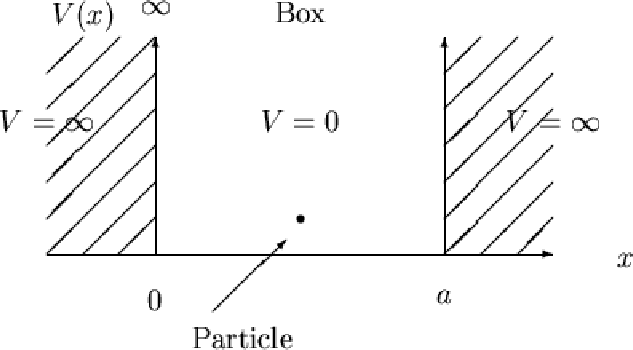
\includegraphics[scale =0.3]{./figures/img53}
	\label{pib}
	\caption{ A diagram illustrating the particle in a box problem}
\end{figure}
This is an idealisation for a large enough potential compared to the particle's energy. This problem is very important example to study discrete spectrum .\\
We start by a particle trapped in a potential well, of width $ a$. The Schr\"{o}dinger's equation for this particle is written as - in position representation-:
\begin{equation}
i \hbar \dfrac{\rd}{\rd t}\psi (x,t) =- \frac{\hbar^2}{2m} \dfrac{ \rd^2}{\rd x^2} \psi(x,t) + V(x) \psi(x,t)
\end{equation}
With :
\begin{equation}
V(x) = \begin{cases}
0, \;  \text { for}\;  0<x<a \\
\infty ,\; \text{ otherwise}
\end{cases}
\end{equation}
Since the above equation is clearly separable, similar to the free particle. It resembles a stationary state. We then write the eigenvalue problem:
\begin{equation}
\frac{\hbar^2}{2m} \dfrac{ \rd^2}{\rd x^2} u(x;E) + V(x) u (x;E) = E u(x; E)
\label{eigen}
\end{equation} 
The energy eigenfunctions  are then equal to $ \psi(x,t ;E) = u(x;E) \; e^{-i\hbar \omega t}$
\subsection{Solution to Schr\"{o}dinger's equation}
We now attempt to solve \eqref{eigen} subject to the boundary conditions:
\begin{equation}
u (x= 0) = u(x=a) = 0
\end{equation}
Because there is a null probability of the particle being outside the box. And the second condition on the wavefunction :
\begin{equation}
\frac{d u(x)}{dx} |_{x = 0} = \frac{d u(x)}{dx}|_{x = a}
\end{equation}
This condition comes from naturally from the analysis of the problem. The first derivative of the wavefunction is proportional to the momentum of the particle, we expect the particle will 'bump' with both walls in the same manner. Although, this  violates the \textit{Born conditions } discussed in lecture 5, but keep in mind that the infinite well is an unphysical example!\\
Now, we rewrite Schr\"{o}dinger's equation as:
\begin{equation}
\frac{d^ 2 u(x)}{dx^ 2}+ k^ 2 u(x) =0
\end{equation}
with $ k = \sqrt{2mE}\hbar $; this differential equation is solved by the substitution $ u (x)= e^{Rx}$ Resulting:
\begin{equation}
u(x) = A e^ {ikx} + Be^{-ikx}
\end{equation}
Where $ A$ and $ B$ are constants, we use the identity :

We observe that, using the boundary conditions we obtain :
\begin{gather}
\begin{align}
ik\left( A e^ {ika} - Be^{-ika} \right)  &= ik (A-B) \nonumber \\
\Rightarrow u(x) = C \sin (kx)
\end{align}
\\
\begin{align}
u(a)& =C\sin(ka) =0  \nonumber \\
\Rightarrow & k = \frac{n \pi}{a}
\end{align}
\end{gather}
But since $ k = \sqrt{2mE}\hbar $, we conclude that energy takes discrete values :
\begin{align}
E_n =& \frac{\hbar^ 2 n^ 2 \pi ^2 }{2m a ^2 } \nonumber \\
=& E_0 \;  n^ 2 
\end{align}
With $ E_0 = \frac{\hbar^ 2  \pi ^2 }{2m a ^2 }$, the ground energy. And $ n$ here denotes the \textbf{quantum number } for the excited states of the particle in the box. Now, we may write the energy-eigenfunctions, after calculating the normalisation factor $ C = \sqrt{\frac{2}{a}} e^{i\varphi}$ \footnote{ we can always add  an arbitrary phase factor $e^{i\varphi}$}
\begin{equation}
\psi_n(x,t) = \sqrt{\frac{2}{a}} \left( \sin(\frac{n \pi x}{a})\right) e^ { i\left( \omega t+\phi\right) }
\end{equation}
The total wavefunction is written as, by the superposition principle :
\begin{equation}
\psi (x,t) = \sqrt{\frac{2}{a}}\sum _{n=1}^ { \infty} \left( \sin(\frac{n \pi x}{a})\right) e^ { i\left( \omega t+\phi\right) }
\end{equation}
Which is a Fourier series ( we could have obtained this solution immediately by Fourier analysis ).
The following figure demonstrates the eigenfunctions for various excitation states, and the probability density function $ \rho$:
\begin{figure}
	\centering
	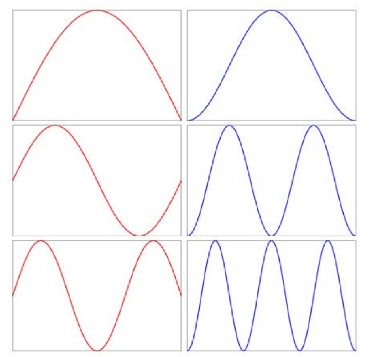
\includegraphics[scale =0.5]{./figures/states}
	\label{s}
	\caption{ First,second, and	third lowest-energy	eigenfunctions (red) and associated probability densities (blue) for the infinite	square well	potential}
\end{figure}
\subsection{Momentum eigenfucntions}
We now turn into calculation the Fourier transform of $ u(x)$ in order to compute the momentum eigenfucntions $ \phi(p,t) $:
\begin{equation}
v(p) = \frac{1}{\sqrt{2 \pi \hbar}} \int_0 ^ a  dx \underbrace{ e^{\frac{i}{\hbar} px}}_{\langle p| x\rangle} \underbrace{u(x)}_{\langle x| u\rangle}
\end{equation}
substituting with $ u(x)$ we have:
\begin{equation}
v(p) =  \frac{1}{\sqrt{ \pi a \hbar}} \int_0 ^ a  dx \;  e^{\frac{i}{\hbar} px} \; \sin ( n \hbar p x )
\end{equation}
Evaluation of this integral gives: \footnote{ The following identity was used : \\ $ \int e^{ax}\, \sin bx\, dx = \frac{ e^{ax}}{a^2 +b^2}\left( a \sin bx + b \cos bx\right) $}
\begin{equation}
v(p) = n \sqrt{\frac{a \pi}{\hbar}}\left( \frac{1-(-1)^n \; e^{-\frac{i}{\hbar}p a}}{n^2 \pi^2 - a^2 \frac{p^2}{\hbar ^2}} \right) 
\end{equation}
Plotting the momentum probability density function  - for various excitations - :
\begin{figure}[h!]
	\centering
	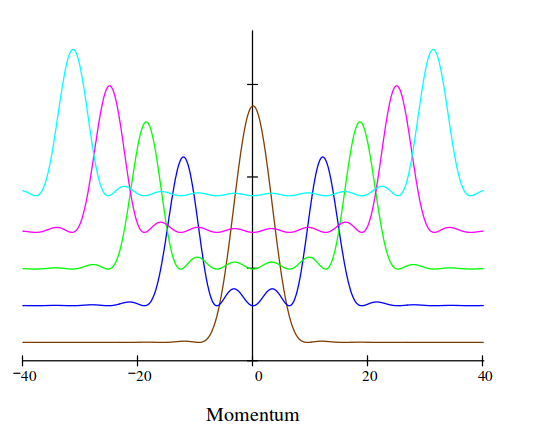
\includegraphics[scale =0.5]{./figures/mom}
	\label{m}
	\caption{ Momentum probability density function for the ground state and three more excitation states.}
\end{figure}
This calculation ends the basic analysis for a particle in a box.
\section{Simple Harmonic Oscillator}
\subsection{Quantization of the SHO Hamiltonian }
From lecture (1) we have the classical Hamiltonian for the simple harmonic oscillator (SHO) :
\begin{equation}
H(p,x)= \frac{1}{2m} p^2 +\frac{1}{2} m\omega^2x^2
\end{equation} 
Using the postulates of quantum mechanics discussed before, we obtain- upon quantization - the Hamiltonian operator 
\begin{equation}
\hat{H}= \frac{1}{2m} \hat{P}^2 +\frac{1}{2} m\omega^2\hat{X}^2
\end{equation}
The Hilbert space of which $\hat{X}$ and $\hat{P}$ act on is\[ \mathcal{L}^2 (-\infty,+\infty; dx)
\]
We now introduce the dimensionless Hamiltonian 
\begin{equation}
\hat{H}'= \frac{1}{2m \hbar \omega } \hat{P}^2 +\frac{1}{2} \frac{m \omega}{\hbar}\hat{X}^2
\end{equation}
This operator can be factorised and written in terms of 'creation' and 'inhalation 'operators; $ a^\dagger$ and $ a$ respectively 
\begin{equation}
\hat{H}'= a^\dagger a + \frac{1}{2} I
\end{equation}
with:
\begin{subequations}
	\begin{align}
	a = & \sqrt{\frac{m\omega}{2\hbar}} \hat{X}+ i \sqrt{\frac{1}{2m\omega \hbar}} \hat{P}\\
	a^\dagger = & \sqrt{\frac{m\omega}{2\hbar}} \hat{X}- i \sqrt{\frac{1}{2m\omega \hbar}} \hat{P}
	\end{align}
\end{subequations}
These operators, along with $\hat{H}'$, satisfy a well-known commutation relations. \footnote{ The operators $a$, $a^\dagger$ and $ H'$ along with the commutator operation $[ \cdot,\cdot]$ satisfy the $su(1,1)$ algebra.}
\begin{subequations}
	\begin{gather}
	[ a, a^\dagger] = I \\
	[a,H'] = a \\
	[a^\dagger,H'] = -a ^\dagger 
	\end{gather}
\end{subequations}
We also define the \textbf{number operator} $ N \equiv a^\dagger a$ that acts on the eigenstates $ |n\rangle$ resulting an eigenvalue of $n$ :
\[
N | n\rangle = n |n\rangle
\]
as a result we may conclude that 
\begin{equation}
a |0\rangle = 0 
\label{inh}
\end{equation}
acting on the 'ground state'by the inhalation operator, kills it.  Moreover 
\begin{gather}
a |n\rangle = \sqrt{n} | n-1\rangle \\
a^\dagger |n\rangle = \sqrt{(n+1)} | n+1\rangle
\end{gather}

Hence, The Hamiltonian acting on these states will result (the energy eigenvalue) 
\begin{equation}
\hat{H} |n\rangle = \hbar \omega (n+\frac{1}{2}) |n\rangle
\end{equation}
Implying that the 'number states' are the excitation states for the quantum harmonic oscillator. The creation and inhalation operators excite or deceit it, and it has a discrete energy spectrum of :
\begin{equation}
E_n = \hbar \omega \left( n+ \frac{1}{2}\right) 
\end{equation}  
Even in the ground state, the quantum harmonic oscillator has a non-vanishing energy. This is a direct result for the uncertainty principle in time and energy. 
\begin{figure}[h!]
	\centering
	
	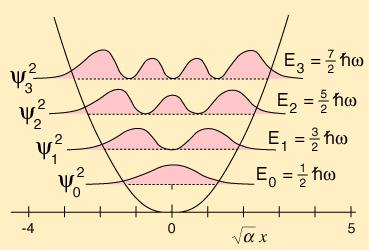
\includegraphics[scale= .7]{./figures/qsho}
	\caption{Energy-levels and wavefunctions of the quantum harmonic oscillator }
\end{figure}
\subsection{The eigenfunctions}
Since we introduced the eigenstates for the Hamiltonian ( or the number operator equivalently). $ | n\rangle$. We can use the ladder operator method to solve Scr\"{o}dinger's equation in the position representation and find $ \psi_n(x) = \langle x| n\rangle$. \\ we start from \eqref{inh}:
\begin{equation}
a \psi_0(x) =0
\end{equation}
resulting the differential equation,
\begin{equation}
\left( x+\frac{\hbar}{m \omega} \frac{d}{dx}\right)  \psi_0(x) =0
\end{equation}
having the solution:
\begin{equation}
\psi_0(x) = A e^{-\frac{m \omega}{2 \hbar} x^2}
\end{equation}
We can find the normalisation factor by:
\begin{equation}
\int_{- \infty}^{+ \infty} e^{-\frac{m \omega}{2 \hbar} x^2} dx = \frac{1}{|A|^2}.
\end{equation}
Which is a typical Gaussian, hence $A$ is found to be,
\begin{equation}
A= \left( \frac{m \omega}{\pi \hbar}\right) ^ {1/4}
\end{equation} 
Now, in order to find the nth wavefunction $ \psi_n(x)$, we first need to prove the following identity
\begin{equation}
| n\rangle = \frac{ (a^\dagger)^n}{\sqrt{n !}} | 0\rangle
\end{equation}
Proof:
\begin{align*}
\frac{a^\dagger}{\sqrt{n}} \mid n - 1 \rangle = \frac{(a^\dagger)^2}{\sqrt{n(n - 1)}}\mid n - 2 \rangle = \cdots = \frac{(a^\dagger)^n}{\sqrt{n!}}|0\rangle.
\end{align*}
Thereby, 
\begin{equation}
\psi_n(x) = \frac{ (a^\dagger)^n}{\sqrt{n !}} \psi_0{x}
\end{equation}
Writing the expression explicitly , we obtain :
\begin{equation}
\psi_n(x)\equiv \left\langle x \mid n \right\rangle = {1 \over \sqrt{2^n n!}}~ \pi^{-1/4} \exp(-x^2 / 2) H_n(x)
\end{equation}
Where $ H_n(x)$ is the nth Hermit polynomial, that having the generating formula (Rodrigues's formula)
\begin{equation}
H_n(x)=(-1)^n e^{x^2}\frac{d^n}{dx^n}e^{-x^2}
\end{equation}
They are one of the classical orthogonal polynomials. \\
Note that this result can be obtained by solving immediately the Schr\"{o}dinger's equation (using series solution, or Sturm-Liouville theorem ).
\subsection{Coherent states}
Coherent states are a very important topic in quantum mechanics. Coherent states are quantum states that display an oscillatory behaviour similar to the one displayed in the simple harmonic oscillator. Formally, a coherent state is a state that has a minimum uncertainty, and takes the form ( where $a$ here is the inhalation operator) :
\begin{equation}
a | \alpha\rangle = \alpha | \alpha\rangle
\end{equation}
The ground state  $ |0 \rangle $ is a coherent state. Since it has the minimum ucertainty :
\begin{equation}
\langle \Delta X \rangle _0\langle \Delta P \rangle _0 = \frac{\hbar}{2}
\end{equation}
This is not however the case for the stationary states $ |n\rangle$, as we can show that:
\begin{equation}
\langle \Delta X \rangle _n\langle \Delta P \rangle _n = \frac{\hbar}{2}(2n+1)
\end{equation}
Hence the states $ \alpha \rangle$, the coherent states of the Harmonic oscillator are not stationary states. Their time evolution is important in the classical limit, as it leads to Ernfest theorem, and one can obtain from them the Classical equations of motion for the Harmonic oscillator. Hence the classical harmonic oscillator is the limit for the coherent states $ | \alpha\rangle $, not the states $ |n\rangle $. However the detailed mathematical argument is beyond the scope of this course, the interested reader might want to refer to any Textbook in the references for details.
\section{Problems}
\subsection{Particle in a box}
\begin{enumerate}
	\item Using the uncertainty principle for position and momentum, estimate the ground state energy for an infinite well of width $a$, compare the obtained result with the one found in the lecture. 
	\item Compute $ \langle E \rangle$, $\langle p \rangle$ and $\langle x \rangle$ for the particle in a box. 
	\item Show that the normalisation factor for the particle in a box wavefunction is given by $ \sqrt{\frac{2}{a}} $ 
	\item Show that the eigenfunctions $ u_n(x)$ are orthogonal .
	\item What is the ground state, first excited and second excited states energies for an electron trapped in an infinite well of width $ 1 $ \AA .
\end{enumerate}
\subsection{Simple Harmonic Oscillator}
\begin{enumerate}
	\item Express the position and momentum operators $X$ and $P$ in terms of $a$ and $ a^\dagger$
	\item Verify the commutation relations of the triple $ H', a $ and $ a^\dagger$ stated in the lecture notes, recall the canonical commutation relation $ [ X,P]= i \hbar I$.
	\item Find $ \langle X\rangle$ , $ \langle P\rangle$  , $ \langle X^2\rangle$ and $ \langle P^2\rangle$ .
	\item A quantum harmonic oscillator, in the 2nd excited state, having an energy of $ 2.45 eV$, find its angular frequency , and period.  
	\item Find the eigenfunction $ \psi_1(x)$, and show that it is orthogonal to $ \psi_0(x)$ seen in the lecture.
	\item From problem (3), verify the uncertainty relation for position and momentum . 
	\item  Verify that $ a^\dagger |n\rangle  = \sqrt{n+1} |n+1\rangle $ 
	\item   Write the operators $ a$ and $a^\dagger$ as matrices  acting on the vector states :
	\[ |0\rangle = \begin{pmatrix}
	1\\0\\0\\ \vdots
	\end{pmatrix} \; \; \; \; \; \; \; |1\rangle = \begin{pmatrix}
	0\\1\\0\\ \vdots
	\end{pmatrix} \; \; \; \; \; \;  |2\rangle = \begin{pmatrix}
	0\\0\\1\\ \vdots
	\end{pmatrix} \dots \]
\end{enumerate}
\nocite{*} 